%%%%%%%%%%%%%%%%%%%%%%%%%%%%%%%%%%%%%%%%%%%%%%%%%%%%%%%%%%%%%%%%%
% Credit Scoring Primer v2.0
% A comprehensive guide to FICO scoring
% LaTeX version with improved formatting
%%%%%%%%%%%%%%%%%%%%%%%%%%%%%%%%%%%%%%%%%%%%%%%%%%%%%%%%%%%%%%%%%

\documentclass[11pt,letterpaper]{article}

% ============== PACKAGES ==============
\usepackage[utf8]{inputenc}
\usepackage[T1]{fontenc}
\usepackage{lmodern}
\usepackage[margin=1in]{geometry}
\usepackage{xcolor}
\usepackage{graphicx}
\usepackage{booktabs}
\usepackage{array}
\usepackage{tabularx}
\usepackage{longtable}
\usepackage{multirow}
\usepackage{colortbl}
\usepackage{hyperref}
\usepackage{titlesec}
\usepackage{enumitem}
\usepackage{tcolorbox}
\usepackage{fancyhdr}
\usepackage{tikz}
\usetikzlibrary{shapes.geometric, arrows.meta, positioning}
\usepackage{fontawesome5}
\usepackage{parskip}
\usepackage{float}
\usepackage{wrapfig}
\usepackage{mdframed}
\usepackage{caption}

% ============== COLORS ==============
\definecolor{primaryblue}{HTML}{1E3A5F}
\definecolor{secondaryblue}{HTML}{2E86AB}
\definecolor{accentgreen}{HTML}{28A745}
\definecolor{accentorange}{HTML}{FD7E14}
\definecolor{accentred}{HTML}{DC3545}
\definecolor{lightgray}{HTML}{F8F9FA}
\definecolor{mediumgray}{HTML}{6C757D}
\definecolor{darkgray}{HTML}{343A40}
\definecolor{tableheader}{HTML}{2E86AB}
\definecolor{tablerow1}{HTML}{FFFFFF}
\definecolor{tablerow2}{HTML}{F0F7FB}
\definecolor{warningbg}{HTML}{FFF3CD}
\definecolor{warningborder}{HTML}{FFC107}
\definecolor{infobg}{HTML}{D1ECF1}
\definecolor{infoborder}{HTML}{17A2B8}
\definecolor{successbg}{HTML}{D4EDDA}
\definecolor{successborder}{HTML}{28A745}
\definecolor{dangerbg}{HTML}{F8D7DA}
\definecolor{dangerborder}{HTML}{DC3545}

% ============== HYPERREF SETUP ==============
\hypersetup{
    colorlinks=true,
    linkcolor=primaryblue,
    urlcolor=secondaryblue,
    citecolor=primaryblue,
    pdftitle={Credit Scoring Primer v2.0},
    pdfauthor={Birdman / Credit Rebels},
    bookmarks=true,
    bookmarksopen=true,
}

% ============== HEADER/FOOTER ==============
\pagestyle{fancy}
\fancyhf{}
\fancyhead[L]{\textcolor{mediumgray}{\small Credit Scoring Primer v2.0}}
\fancyhead[R]{\textcolor{mediumgray}{\small Credit Rebels}}
\fancyfoot[L]{\textcolor{mediumgray}{\small\nouppercase{\leftmark}}}
\fancyfoot[R]{\textcolor{mediumgray}{\thepage}}
\renewcommand{\headrulewidth}{0.4pt}
\renewcommand{\footrulewidth}{0.4pt}

% ============== SECTION FORMATTING ==============
\titleformat{\section}
    {\normalfont\Large\bfseries\color{primaryblue}}
    {\thesection.}{0.5em}{}
    [\titlerule]

\titleformat{\subsection}
    {\normalfont\large\bfseries\color{secondaryblue}}
    {\thesubsection}{0.5em}{}

\titleformat{\subsubsection}
    {\normalfont\normalsize\bfseries\color{darkgray}}
    {\thesubsubsection}{0.5em}{}

\titlespacing*{\section}{0pt}{2ex plus 1ex minus .2ex}{1.5ex plus .2ex}
\titlespacing*{\subsection}{0pt}{1.5ex plus 1ex minus .2ex}{1ex plus .2ex}
\titlespacing*{\subsubsection}{0pt}{1ex plus 1ex minus .2ex}{0.5ex plus .2ex}

% ============== CUSTOM BOXES ==============
\newtcolorbox{keypoint}{
    colback=infobg,
    colframe=infoborder,
    fonttitle=\bfseries,
    title={\faIcon{key} Key Point},
    rounded corners,
    boxrule=1pt,
    left=10pt,
    right=10pt,
    top=5pt,
    bottom=5pt
}

\newtcolorbox{warning}{
    colback=warningbg,
    colframe=warningborder,
    fonttitle=\bfseries,
    title={\faIcon{exclamation-triangle} Warning},
    rounded corners,
    boxrule=1pt,
    left=10pt,
    right=10pt,
    top=5pt,
    bottom=5pt
}

\newtcolorbox{optimal}{
    colback=successbg,
    colframe=successborder,
    fonttitle=\bfseries,
    title={\faIcon{check-circle} Optimal Value},
    rounded corners,
    boxrule=1pt,
    left=10pt,
    right=10pt,
    top=5pt,
    bottom=5pt
}

\newtcolorbox{danger}{
    colback=dangerbg,
    colframe=dangerborder,
    fonttitle=\bfseries,
    title={\faIcon{times-circle} Avoid},
    rounded corners,
    boxrule=1pt,
    left=10pt,
    right=10pt,
    top=5pt,
    bottom=5pt
}

\newtcolorbox{definition}{
    colback=lightgray,
    colframe=mediumgray,
    fonttitle=\bfseries,
    title={\faIcon{book} Definition},
    rounded corners,
    boxrule=1pt,
    left=10pt,
    right=10pt,
    top=5pt,
    bottom=5pt
}

% ============== CUSTOM COMMANDS ==============
\newcommand{\threshold}[1]{\textcolor{accentorange}{\textbf{#1}}}
\newcommand{\fico}{FICO\textsuperscript{\textregistered}}
\newcommand{\term}[1]{\textcolor{secondaryblue}{\textbf{#1}}}
\newcommand{\acronym}[2]{\textbf{#1} (#2)}

% ============== DOCUMENT START ==============
\begin{document}

% ============== TITLE PAGE ==============
\begin{titlepage}
    \centering
    \vspace*{1cm}

    {\Huge\bfseries\color{primaryblue} Credit Scoring Primer}\\[0.5cm]
    {\LARGE\color{secondaryblue} Version 2.0}\\[1.5cm]

    % Credit Score Gauge
    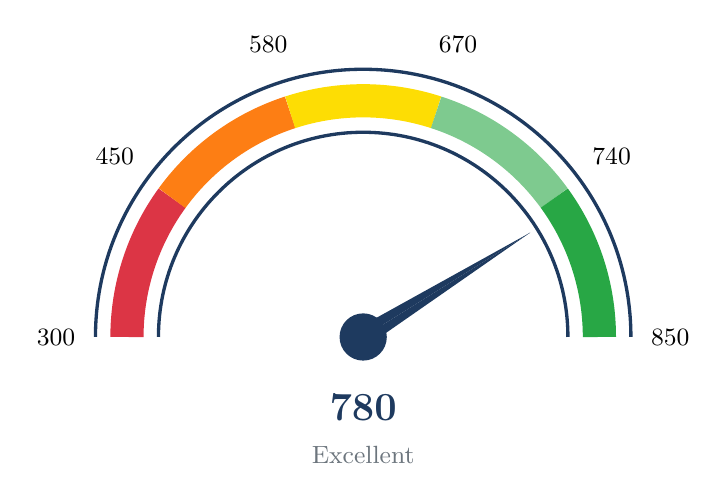
\begin{tikzpicture}
        % Gauge arc with color gradient
        \draw[line width=12pt, accentred] (180:3cm) arc (180:144:3cm);
        \draw[line width=12pt, accentorange] (144:3cm) arc (144:108:3cm);
        \draw[line width=12pt, yellow!80!orange] (108:3cm) arc (108:72:3cm);
        \draw[line width=12pt, accentgreen!60] (72:3cm) arc (72:36:3cm);
        \draw[line width=12pt, accentgreen] (36:3cm) arc (36:0:3cm);

        % Outer arc border
        \draw[primaryblue, very thick] (180:3.4cm) arc (180:0:3.4cm);
        \draw[primaryblue, very thick] (180:2.6cm) arc (180:0:2.6cm);

        % Score labels
        \node at (180:3.9cm) {\small 300};
        \node at (144:3.9cm) {\small 450};
        \node at (108:3.9cm) {\small 580};
        \node at (72:3.9cm) {\small 670};
        \node at (36:3.9cm) {\small 740};
        \node at (0:3.9cm) {\small 850};

        % Needle pointing to excellent score
        \fill[primaryblue] (0,0) -- (32:2.5cm) -- (0,0.15) -- cycle;
        \fill[primaryblue] (0,0) -- (32:2.5cm) -- (0,-0.15) -- cycle;
        \fill[primaryblue] (0,0) circle (0.3cm);

        % Score display
        \node at (0,-0.9) {\Large\bfseries\color{primaryblue} 780};
        \node at (0,-1.5) {\small\color{mediumgray} Excellent};
    \end{tikzpicture}\\[1.5cm]

    {\large\itshape In memoriam}\\[0.3cm]
    {\Large\bfseries Birdman, Birdman7, MFBirdman7}\\[0.2cm]
    {\large (1976 -- 2023)}\\[1.5cm]

    
\begin{tikzpicture}
        \draw[primaryblue, line width=2pt] (0,0) -- (10,0);
    \end{tikzpicture}\\[1cm]

    {\large Last Update: Friday, May 26, 2023 EDT}\\[0.5cm]

    \vfill

    {\Large\color{secondaryblue}\textbf{Credit Rebels}}\\[0.5cm]
    {\small The most accurate and comprehensive publication on \fico{} scoring available today}

\end{titlepage}

% ============== TABLE OF CONTENTS ==============
\tableofcontents
\newpage

% ============== INTRODUCTION ==============
\section{Introduction}

Welcome to the best-kept secret in the credit-scoring world! If you are in-the-know, welcome back! If this is your first encounter, well brace yourself and pack a lunch! This is Version 2.0 of the already-famous Credit Scoring Primer!

\fico{} algorithms play a major role in the credit world. One of their many variants of scoring algorithms is sure to play a part in your next credit attempt, so the knowledge of how to maximize that score is invaluable when seeking/using credit.

\begin{keypoint}
This document represents the most accurate and comprehensive publication on \fico{} scoring available today. It's lengthy, detailed, and complex---but if you're committed and determined, it will be one of the most enlightening journeys you have ever taken.
\end{keypoint}

Please keep in mind the Credit Scoring Primer is composed with a very knowledgeable, technical audience in mind. If you feel overwhelmed, take it one section at a time and read each section repeatedly until you internalize it.

% ============== QUICK REFERENCE TABLE ==============
\section{Quick Reference: FICO Score 8 Optimal Attributes}

\begin{table}[H]
\centering
\caption{\fico{} Score 8 Select Optimal Characteristic Attributes}
\label{tab:optimal-attributes}
\rowcolors{2}{tablerow2}{tablerow1}
\begin{tabularx}{\textwidth}{>{\bfseries}l X}
\toprule
\rowcolor{tableheader}
\textcolor{white}{\textbf{Characteristic}} & \textcolor{white}{\textbf{Optimal Attribute}} \\
\midrule
Payment History & 100\%, Zero baddies. Penalty fully removed after 7 years. 60D late or worse = dirty scorecard. \\
\addlinespace
Aggregate Utilization & \threshold{<9.5\%} (or <4.5\% for both individual and aggregate revolving on some scorecards) \\
\addlinespace
Retail Utilization & \threshold{\$0} \\
\addlinespace
Accounts with Balance (AWB) & \threshold{<20\%} AWB recommended. Metric weighted less in Score 8. \\
\addlinespace
Bankcards with Balance (BWB) & The lower, the better (under study) \\
\addlinespace
Revolving Balance & \threshold{<\$1000} for 8/9; Never \$0 (All Zero loss of 10--25 points) \\
\addlinespace
AoOA (Oldest Account) & \textbf{Not} a scoring factor. Segmentation factor: 36 months for 8/9 \\
\addlinespace
AoORA (Oldest Revolver) & Scoring factor. 20 years reported to max. \\
\addlinespace
AAoA (Avg Age of Accounts) & Max award believed by \threshold{90 months} \\
\addlinespace
AAoRA (Avg Age Revolvers) & 9 years reported to max \\
\addlinespace
AoYA (Youngest Account) & Awards at multiples of 3 months possibly \\
\addlinespace
AoYRA (Youngest Revolver) & Segmentation factor at \threshold{12 months}; ~10--20 points \\
\addlinespace
Inquiries (Last 12 Months) & \threshold{Zero}. Penalty removed at 365 days. \\
\addlinespace
Total Accounts/Mix & \textbf{Not} a scoring factor. 4 TLs for Thick. Include 1 loan for diversity. \\
\addlinespace
Number of Bankcards & Optimal unknown. 5--7? Loss for <3. \\
\bottomrule
\end{tabularx}
\end{table}

% ============== BACKGROUND ==============
\section{Background}

\subsection{Origins of This Document}

MWGardener19 had the idea for a Score 8 Master Thread. He produced an intro and a small Reddit post---``\fico{} reverse engineered''---by u/rtanaka6 who had composed it from years of reading myFICO forums. It had many inaccuracies and so much was missing. Birdman went crazy correcting, adding, and expanding, and this is where it ended up: a new creation, the Credit Scoring Primer.

\subsection{Brief History of FICO}

\begin{itemize}[leftmargin=*]
    \item Fair Isaac and Company (\fico{}) states \textbf{Score 8} is the most widely used credit scoring system
    \item Score 8 is one of many models: Score 2, 3, 4, 8, 9; Bankcard 2, 3, 4, 5, 8, 9; Auto Score 2, 4, 5, 8, 9
    \item \fico{} began creating systems over 60 years ago (1956)
    \item The modern \fico{} scoring system is about 30 years old (1989)
    \item \fico{} is a large, global, publicly owned company with over 4000 employees
    \item 88\% of \$1 billion revenue comes from banking/insurance customers
\end{itemize}

\subsection{What We Know About FICO Scoring}

\begin{keypoint}
\begin{itemize}[leftmargin=*]
    \item We have come to know \textbf{GENERALLY} how \fico{} scoring works
    \item We have come to know \textbf{A LOT} about how certain aspects of scoring works
    \item We have come to know that we do \textbf{NOT} know \textbf{EXACTLY} how all of \fico{} scoring works
\end{itemize}
\end{keypoint}

\fico{}'s approach to performing credit scoring is proprietary. The underlying math considers Lorenz curves, Gini coefficients, normalized log Bernoulli Likelihood, multicollinearity testing, and other higher mathematics.

% ============== SCORE RATINGS ==============
\subsection{FICO Score 8 Ratings}

\begin{table}[H]
\centering
\caption{\fico{} Score 8 Rating Categories}
\rowcolors{2}{tablerow2}{tablerow1}
\begin{tabular}{lcc}
\toprule
\rowcolor{tableheader}
\textcolor{white}{\textbf{Rating}} & \textcolor{white}{\textbf{Score Range}} & \textcolor{white}{\textbf{Indicator}} \\
\midrule
Exceptional & 800 -- 850 & \textcolor{accentgreen}{\faIcon{star}\faIcon{star}\faIcon{star}\faIcon{star}\faIcon{star}} \\
Very Good & 740 -- 799 & \textcolor{accentgreen}{\faIcon{star}\faIcon{star}\faIcon{star}\faIcon{star}} \\
Good & 670 -- 739 & \textcolor{accentorange}{\faIcon{star}\faIcon{star}\faIcon{star}} \\
Fair & 580 -- 669 & \textcolor{accentorange}{\faIcon{star}\faIcon{star}} \\
Poor & 300 -- 579 & \textcolor{accentred}{\faIcon{star}} \\
\bottomrule
\end{tabular}
\end{table}

% ============== FIVE CATEGORIES ==============
\subsection{The Five Scoring Categories}

\begin{table}[H]
\centering
\caption{Scoring Categories and Typical Weightings}
\rowcolors{2}{tablerow2}{tablerow1}
\begin{tabular}{clcc}
\toprule
\rowcolor{tableheader}
\textcolor{white}{\textbf{\#}} & \textcolor{white}{\textbf{Category}} & \textcolor{white}{\textbf{Weight}} & \textcolor{white}{\textbf{~Points}} \\
\midrule
1 & Payment History & 35\% & ~192.5 \\
2 & Amount of Debt & 30\% & ~165 \\
3 & Length of History & 15\% & ~82.5 \\
4 & New Credit & 10\% & ~55 \\
5 & Credit Mix & 10\% & ~55 \\
\bottomrule
\end{tabular}
\end{table}

% ============== SCORECARD BASICS ==============
\section{Scorecard Basics}

\begin{definition}
\textbf{Characteristics} are metrics within each category. \fico{} calls each metric a ``characteristic'' and the corresponding value is called an ``attribute.''
\begin{itemize}[leftmargin=*]
    \item \textbf{Segmentation Factors}: Determine which scorecard you're assigned to
    \item \textbf{Scoring Factors}: Directly affect your score; weighting varies by scorecard
\end{itemize}
\end{definition}

\subsection{Score 8 Scorecards Overview}

Score 8 has \textbf{12 scorecards}: 8 clean and 4 dirty scorecards.

\begin{table}[H]
\centering
\caption{Scorecard Segmentation Factors}
\begin{tabular}{ll}
\toprule
\rowcolor{tableheader}
\textcolor{white}{\textbf{Profile Type}} & \textcolor{white}{\textbf{Segmentation Factors}} \\
\midrule
\rowcolor{tablerow2}
\textbf{Clean Profiles} & Thick/Thin (number of accounts) \\
\rowcolor{tablerow2}
 & Mature/Young (age of oldest account) \\
\rowcolor{tablerow2}
 & No New Revolver/New Revolver (recency) \\
\midrule
\rowcolor{tablerow1}
\textbf{Dirty Profiles} & PR/No PR (severity) \\
\rowcolor{tablerow1}
 & Recent/Mature (recency) \\
\bottomrule
\end{tabular}
\end{table}

\subsection{Scorecard Segmentation Diagram}

\begin{figure}[H]
\centering
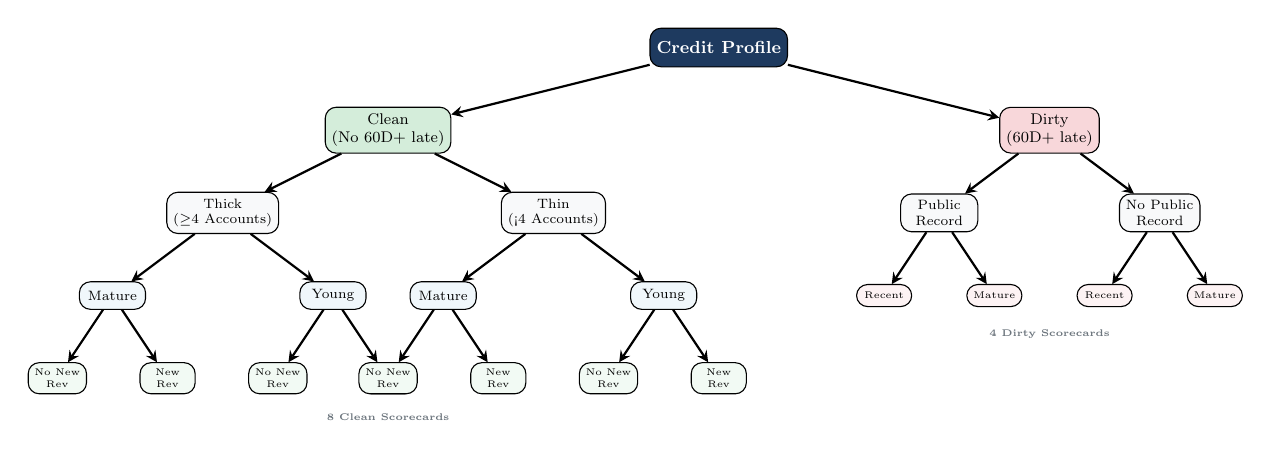
\begin{tikzpicture}[scale=0.7, transform shape]
    % Styles
    \tikzstyle{root} = [draw, rounded corners, fill=primaryblue, text=white, minimum width=2cm, minimum height=0.7cm, align=center, font=\small\bfseries]
    \tikzstyle{level1} = [draw, rounded corners, minimum width=1.6cm, minimum height=0.6cm, align=center, font=\footnotesize]
    \tikzstyle{level2} = [draw, rounded corners, minimum width=1.4cm, minimum height=0.5cm, align=center, font=\scriptsize]
    \tikzstyle{level3} = [draw, rounded corners, minimum width=1.2cm, minimum height=0.5cm, align=center, font=\scriptsize]
    \tikzstyle{leaf} = [draw, rounded corners, minimum width=1cm, minimum height=0.4cm, align=center, font=\tiny]
    \tikzstyle{arrow} = [draw, ->, >=stealth, thick]

    % Root
    \node[root] (root) at (0,0) {Credit Profile};

    % Level 1: Clean/Dirty
    \node[level1, fill=successbg] (clean) at (-6,-1.5) {Clean\\(No 60D+ late)};
    \node[level1, fill=dangerbg] (dirty) at (6,-1.5) {Dirty\\(60D+ late)};

    % Level 2: Thick/Thin for Clean, Public Record/No PR for Dirty
    \node[level2, fill=lightgray] (thick) at (-9,-3) {Thick\\($\geq$4 Accounts)};
    \node[level2, fill=lightgray] (thin) at (-3,-3) {Thin\\(<4 Accounts)};
    \node[level2, fill=lightgray] (pr) at (4,-3) {Public\\Record};
    \node[level2, fill=lightgray] (nopr) at (8,-3) {No Public\\Record};

    % Level 3: Mature/Young
    \node[level3, fill=tablerow2] (tm) at (-11,-4.5) {Mature};
    \node[level3, fill=tablerow2] (ty) at (-7,-4.5) {Young};
    \node[level3, fill=tablerow2] (thm) at (-5,-4.5) {Mature};
    \node[level3, fill=tablerow2] (thy) at (-1,-4.5) {Young};

    % Level 4: New Revolver/No New Revolver (8 clean scorecards)
    \node[leaf, fill=successbg!30] (tm-nnr) at (-12,-6) {No New\\Rev};
    \node[leaf, fill=successbg!30] (tm-nr) at (-10,-6) {New\\Rev};
    \node[leaf, fill=successbg!30] (ty-nnr) at (-8,-6) {No New\\Rev};
    \node[leaf, fill=successbg!30] (ty-nr) at (-6,-6) {New\\Rev};
    \node[leaf, fill=successbg!30] (thm-nnr) at (-6,-6) {No New\\Rev};
    \node[leaf, fill=successbg!30] (thm-nr) at (-4,-6) {New\\Rev};
    \node[leaf, fill=successbg!30] (thy-nnr) at (-2,-6) {No New\\Rev};
    \node[leaf, fill=successbg!30] (thy-nr) at (0,-6) {New\\Rev};

    % Dirty scorecards (4 total)
    \node[leaf, fill=dangerbg!30] (pr-r) at (3,-4.5) {Recent};
    \node[leaf, fill=dangerbg!30] (pr-m) at (5,-4.5) {Mature};
    \node[leaf, fill=dangerbg!30] (nopr-r) at (7,-4.5) {Recent};
    \node[leaf, fill=dangerbg!30] (nopr-m) at (9,-4.5) {Mature};

    % Arrows
    \draw[arrow] (root) -- (clean);
    \draw[arrow] (root) -- (dirty);
    \draw[arrow] (clean) -- (thick);
    \draw[arrow] (clean) -- (thin);
    \draw[arrow] (dirty) -- (pr);
    \draw[arrow] (dirty) -- (nopr);
    \draw[arrow] (thick) -- (tm);
    \draw[arrow] (thick) -- (ty);
    \draw[arrow] (thin) -- (thm);
    \draw[arrow] (thin) -- (thy);
    \draw[arrow] (tm) -- (tm-nnr);
    \draw[arrow] (tm) -- (tm-nr);
    \draw[arrow] (ty) -- (ty-nnr);
    \draw[arrow] (ty) -- (ty-nr);
    \draw[arrow] (thm) -- (thm-nnr);
    \draw[arrow] (thm) -- (thm-nr);
    \draw[arrow] (thy) -- (thy-nnr);
    \draw[arrow] (thy) -- (thy-nr);
    \draw[arrow] (pr) -- (pr-r);
    \draw[arrow] (pr) -- (pr-m);
    \draw[arrow] (nopr) -- (nopr-r);
    \draw[arrow] (nopr) -- (nopr-m);

    % Labels
    \node[font=\tiny, text=mediumgray] at (-6,-6.7) {\textbf{8 Clean Scorecards}};
    \node[font=\tiny, text=mediumgray] at (6,-5.2) {\textbf{4 Dirty Scorecards}};
\end{tikzpicture}
\caption{Score 8 Scorecard Segmentation Tree (12 Total Scorecards)}
\end{figure}

\begin{warning}
\textbf{Scorecard Reassignment (Rebucketing):} When you change scorecards, your score can boost or drop significantly. Moving to a ``higher'' scorecard often means a score \textit{drop} because you're now compared to a subpopulation with better credit profiles. Most experience a significant drop at 3 years AoOA when reassigned to a mature scorecard.
\end{warning}

% ============== PAYMENT HISTORY ==============
\section{Payment History Category (Clean/Dirty)}

\begin{center}
\colorbox{primaryblue}{\textcolor{white}{\textbf{\Large 35\% of Score $\approx$ 192.5 Points}}}
\end{center}

\subsection{Seven Components of Payment History}

\begin{enumerate}[leftmargin=*]
    \item \textbf{Payment information} on all tradelines (credit cards, retail accounts, installment loans, mortgages)
    \item \textbf{Severity}: How overdue delinquent payments are/were
    \item \textbf{Amount} of money still owed on delinquent accounts or collection items
    \item \textbf{Frequency}: Number of past due items on credit report
    \item \textbf{Recency}: Time passed since delinquencies, adverse public records, or collections
    \item \textbf{Number} of accounts being paid as agreed
    \item \textbf{Adverse public records} (bankruptcies, etc.)
\end{enumerate}

\subsection{Derogatory Categories}

\begin{danger}
This is the most important category. There can be \textbf{no derogatories} on your file for maximum scoring. The algorithm looks for:
\begin{itemize}[leftmargin=*]
    \item Delinquencies (30, 60, 90, 120 days late)
    \item Charge-offs (CO)
    \item Collections
    \item Bankruptcy
    \item Foreclosures
    \item Repossessions
    \item Tax liens
    \item Consumer Finance Accounts (CFAs)
\end{itemize}
\end{danger}

\begin{keypoint}
A \textbf{60-day late} is considered a major derogatory and will segment you into a \textbf{dirty scorecard for 7 years} on Score 8.
\end{keypoint}

\subsection{Collections and Debt Validation}

\begin{definition}
\textbf{Collection Authority (CA)}: If you fail to pay a debt after charge-off, it could be assigned or sold to a CA. This creates a separate tradeline that causes additional penalty and scorecard reassignment to a PR card.
\end{definition}

\subsubsection{Debt Validation (DV) Process}

\begin{enumerate}[leftmargin=*]
    \item Upon ``initial communication,'' a CA must notify you in writing within 5 days of your DV rights (Dunning Notice)
    \item You have \textbf{30 days} to request DV
    \item Send via \textbf{CMRRR} (Certified Mail Return Receipt Requested)
    \item Until CA responds, they are under a ``cease contact bar''
\end{enumerate}

\begin{warning}
A DV does \textbf{NOT} force a CA to delete. It simply imposes a ``cease contact bar'' until they respond. Don't assume you have the upper hand if they don't respond.
\end{warning}

\subsubsection{Pay for Delete (PFD)}

If the debt is \textit{sold} to a CA, you must negotiate with the CA. Request a \textbf{PFD} (Pay for Delete)---paying in return for deletion. This is against CRA policy but some CAs will accommodate.

\begin{keypoint}
For collections, \fico{} only considers:
\begin{enumerate}
    \item Has a collection appeared on your credit report?
    \item When was it reported?
\end{enumerate}
Whether it's \textit{paid} is not a scoring consideration until Version 9!
\end{keypoint}

\subsection{Derogatory Aging}

\subsubsection{Scoring Impact Over Time}

Delinquency penalties are believed to reduce at:
\begin{itemize}[leftmargin=*]
    \item \threshold{6 months}
    \item \threshold{12 months}
    \item \threshold{18 months}
    \item \threshold{2 years} (scorecard reassignment)
\end{itemize}

All baddies affect score for \textbf{7 years}.

\begin{definition}
\textbf{TPOD (Total Period of Delinquency)}: The score loss appears tied to TPOD, which runs from DOFD (Date of First Delinquency) until last update (if unpaid) or until paid.
\end{definition}

\begin{warning}
\textbf{TPOD Catchup Penalty}: If an unpaid charge-off hasn't been updated regularly, then gets updated later (e.g., when you pay it), the algorithm realizes TPOD has increased and you may see a score \textit{drop}.
\end{warning}

\subsubsection{Credit Report Removal Quick Reference}

\begin{table}[H]
\centering
\caption{FCRA §605(a) Removal Timeframes}
\rowcolors{2}{tablerow2}{tablerow1}
\begin{tabularx}{\textwidth}{lXl}
\toprule
\rowcolor{tableheader}
\textcolor{white}{\textbf{Section}} & \textcolor{white}{\textbf{Item}} & \textcolor{white}{\textbf{Removal Period}} \\
\midrule
§605(a)(1) & Bankruptcy & 10 years from order/adjudication \\
§605(a)(3) & Paid Tax Liens & 7 years from payment \\
§605(a)(4) & Charge-offs and Collections & 7.5 years from DOFD (5 years in NY) \\
§605(a)(5) & Other negative information & 7 years \\
\bottomrule
\end{tabularx}
\end{table}

\begin{figure}[H]
\centering
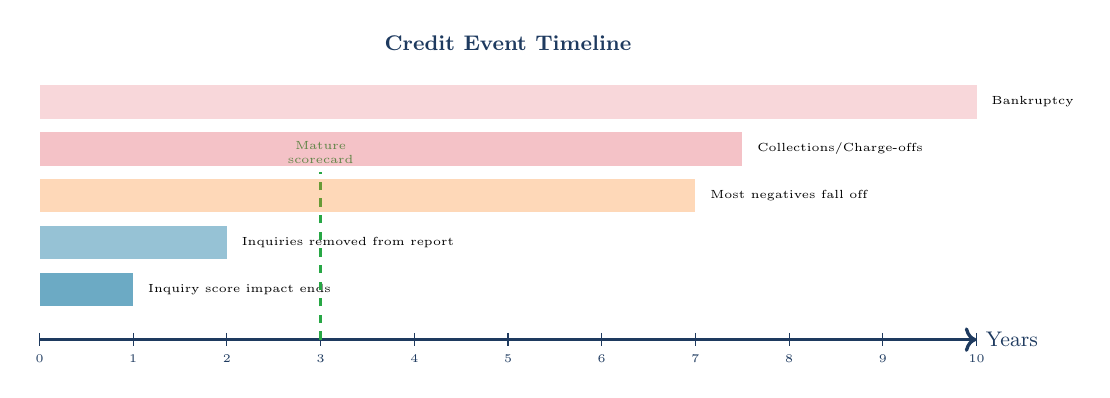
\begin{tikzpicture}[scale=0.85, transform shape]
    % Timeline axis
    \draw[very thick, primaryblue, ->] (0,0) -- (14,0) node[right] {\small Years};

    % Year markers
    \foreach \x/\yr in {0/0, 1.4/1, 2.8/2, 4.2/3, 5.6/4, 7/5, 8.4/6, 9.8/7, 11.2/8, 12.6/9, 14/10} {
        \draw[primaryblue] (\x,0.1) -- (\x,-0.1) node[below] {\tiny\yr};
    }

    % Inquiry score impact (12 months)
    \fill[secondaryblue, opacity=0.7] (0,0.5) rectangle (1.4,1);
    \node[right, font=\tiny] at (1.5,0.75) {Inquiry score impact ends};

    % Inquiry removal (24 months)
    \fill[secondaryblue, opacity=0.5] (0,1.2) rectangle (2.8,1.7);
    \node[right, font=\tiny] at (2.9,1.45) {Inquiries removed from report};

    % AoOA Mature threshold (3 years)
    \draw[accentgreen, very thick, dashed] (4.2,0) -- (4.2,2.5);
    \node[accentgreen, above, font=\tiny, align=center] at (4.2,2.5) {Mature\\scorecard};

    % 7 year mark - most negatives
    \fill[accentorange, opacity=0.3] (0,1.9) rectangle (9.8,2.4);
    \node[right, font=\tiny] at (9.9,2.15) {Most negatives fall off};

    % 7.5 year mark - collections
    \fill[accentred, opacity=0.3] (0,2.6) rectangle (10.5,3.1);
    \node[right, font=\tiny] at (10.6,2.85) {Collections/Charge-offs};

    % 10 year mark - bankruptcy
    \fill[dangerbg] (0,3.3) rectangle (14,3.8);
    \node[right, font=\tiny] at (14.1,3.55) {Bankruptcy};

    % Title
    \node[above, font=\small\bfseries, primaryblue] at (7,4.2) {Credit Event Timeline};
\end{tikzpicture}
\caption{Timeline of Score Impact and Report Removal}
\end{figure}

\subsection{Number of Accounts Paid as Agreed}

\begin{optimal}
A variety of at least \textbf{6 positive accounts}, actively reporting paid as agreed, seems to be the minimum without a loss.
\end{optimal}

% ============== AMOUNT OF DEBT ==============
\section{Amount of Debt Category}

\begin{center}
\colorbox{primaryblue}{\textcolor{white}{\textbf{\Large 30\% of Score $\approx$ 165 Points}}}
\end{center}

\subsection{Utilization}

Utilization metrics are \textbf{scoring factors}.

\subsubsection{Revolving Utilization}

\begin{table}[H]
\centering
\caption{Revolving Utilization Thresholds}
\begin{tabular}{lcc}
\toprule
\rowcolor{tableheader}
\textcolor{white}{\textbf{Type}} & \textcolor{white}{\textbf{Thresholds}} & \textcolor{white}{\textbf{Optimal}} \\
\midrule
\rowcolor{tablerow2}
Aggregate Revolving & 5\%, 10\%, 30\%, 50\%, 70\%, 90\%, 100\% & \textcolor{accentgreen}{\textbf{<9.5\%}} \\
\rowcolor{tablerow1}
Individual Revolving & 30\%, 50\%, 70\%, 90\%, 100\% & \textcolor{accentgreen}{\textbf{<30\%}} \\
\bottomrule
\end{tabular}
\end{table}

\begin{figure}[H]
\centering
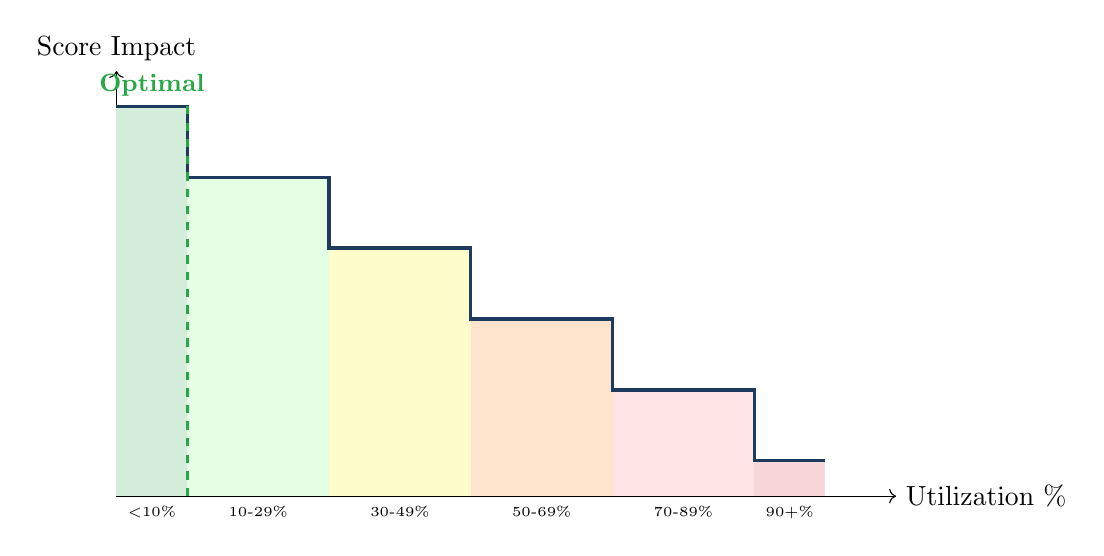
\begin{tikzpicture}[scale=0.9]
    % Draw axes
    \draw[->] (0,0) -- (11,0) node[right] {Utilization \%};
    \draw[->] (0,0) -- (0,6) node[above] {Score Impact};

    % Draw threshold zones
    \fill[successbg] (0,0) rectangle (1,5.5);
    \fill[green!10] (1,0) rectangle (3,4.5);
    \fill[yellow!20] (3,0) rectangle (5,3.5);
    \fill[orange!20] (5,0) rectangle (7,2.5);
    \fill[red!10] (7,0) rectangle (9,1.5);
    \fill[dangerbg] (9,0) rectangle (10,0.5);

    % Draw step function (thresholds deliver full impact at crossing)
    \draw[primaryblue, very thick]
        (0,5.5) -- (1,5.5) -- (1,4.5) -- (3,4.5) -- (3,3.5) -- (5,3.5) -- (5,2.5) -- (7,2.5) -- (7,1.5) -- (9,1.5) -- (9,0.5) -- (10,0.5);

    % Labels
    \node[below] at (0.5,0) {\tiny <10\%};
    \node[below] at (2,0) {\tiny 10-29\%};
    \node[below] at (4,0) {\tiny 30-49\%};
    \node[below] at (6,0) {\tiny 50-69\%};
    \node[below] at (8,0) {\tiny 70-89\%};
    \node[below] at (9.5,0) {\tiny 90+\%};

    % Optimal marker
    \draw[accentgreen, very thick, dashed] (1,0) -- (1,5.5);
    \node[accentgreen, above] at (0.5,5.5) {\small\textbf{Optimal}};
\end{tikzpicture}
\caption{Aggregate Revolving Utilization Impact on Score}
\end{figure}

\subsubsection{Loan Utilization}

\begin{optimal}
The largest threshold (biggest point award) comes when Balance/Limit is \textbf{<9.5\%}. This strategy is worth \textbf{15--35 points}.

\textbf{Strategy}: Get a long-term loan, pay it down to <9.5\%, and do a small amount of auto-pay for activity. Requires a FI that doesn't advance the maturity date.
\end{optimal}

\subsection{Number of Accounts with Balance / AZEO}

The number of accounts reporting a balance impacts score \textbf{independent of utilization}.

\begin{definition}
\textbf{AZEO (All Zero Except One)}: A strategy where only one national bankcard reports a small balance. This guarantees you're below the lowest threshold for the AWB metric.
\end{definition}

\begin{figure}[H]
\centering
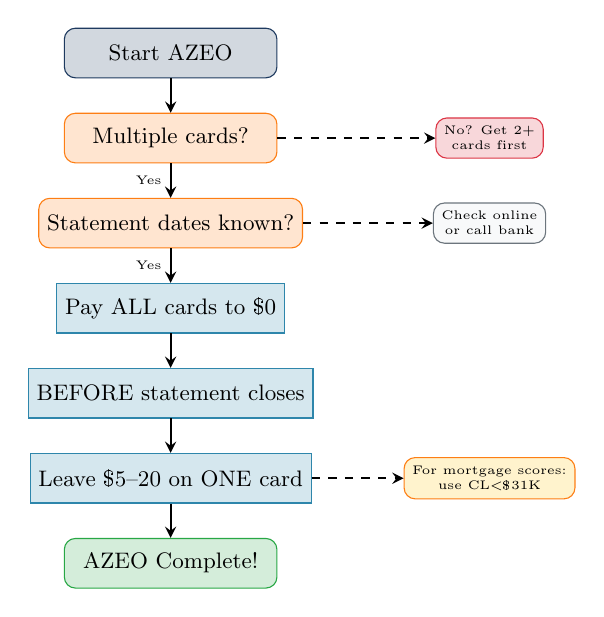
\begin{tikzpicture}[scale=0.9, transform shape]
    % Styles
    \tikzstyle{startstop} = [rectangle, rounded corners, minimum width=3cm, minimum height=0.7cm, text centered, draw=primaryblue, fill=primaryblue!20, font=\small]
    \tikzstyle{process} = [rectangle, minimum width=3cm, minimum height=0.7cm, text centered, draw=secondaryblue, fill=secondaryblue!20, font=\small]
    \tikzstyle{decision} = [rectangle, rounded corners, minimum width=3cm, minimum height=0.7cm, text centered, draw=accentorange, fill=accentorange!20, font=\small]
    \tikzstyle{good} = [rectangle, rounded corners, minimum width=3cm, minimum height=0.7cm, text centered, draw=accentgreen, fill=successbg, font=\small]
    \tikzstyle{arrow} = [thick,->,>=stealth]

    % Nodes - using absolute positioning
    \node[startstop] (start) at (0,0) {Start AZEO};
    \node[decision] (q1) at (0,-1.2) {Multiple cards?};
    \node[decision] (q2) at (0,-2.4) {Statement dates known?};
    \node[process] (step1) at (0,-3.6) {Pay ALL cards to \$0};
    \node[process] (step2) at (0,-4.8) {BEFORE statement closes};
    \node[process] (step3) at (0,-6) {Leave \$5--20 on ONE card};
    \node[good] (end) at (0,-7.2) {AZEO Complete!};

    % Side notes
    \node[draw=accentred, fill=dangerbg, rounded corners, font=\tiny, align=center] (note1) at (4.5,-1.2) {No? Get 2+\\cards first};
    \node[draw=mediumgray, fill=lightgray, rounded corners, font=\tiny, align=center] (note2) at (4.5,-2.4) {Check online\\or call bank};
    \node[draw=accentorange, fill=warningbg, rounded corners, font=\tiny, align=center] (note3) at (4.5,-6) {For mortgage scores:\\use CL<\$31K};

    % Arrows
    \draw[arrow] (start) -- (q1);
    \draw[arrow] (q1) -- node[left, font=\tiny] {Yes} (q2);
    \draw[arrow] (q2) -- node[left, font=\tiny] {Yes} (step1);
    \draw[arrow] (step1) -- (step2);
    \draw[arrow] (step2) -- (step3);
    \draw[arrow] (step3) -- (end);

    % Side arrows
    \draw[arrow, dashed] (q1) -- (note1);
    \draw[arrow, dashed] (q2) -- (note2);
    \draw[arrow, dashed] (step3) -- (note3);
\end{tikzpicture}
\caption{AZEO Strategy Decision Flowchart}
\end{figure}

\begin{optimal}
\textbf{Recommended AZEO Setup:}
\begin{itemize}[leftmargin=*]
    \item Small balance (<4.5\% of CL) on \textbf{one national bankcard}
    \item Credit limit of \textbf{\$30,000 or less} (mortgage scores exclude higher CLs)
    \item Balance of \textbf{\$5--\$20}
    \item \textbf{Avoid}: Retail cards, credit union cards, charge cards
\end{itemize}
\end{optimal}

\begin{warning}
\textbf{Chase users}: Be careful if you pay to \$0---Chase automatically off-cycle updates \$0 balances, which can cause an unintentional All Zero loss.
\end{warning}

\subsection{All Zero Point Loss}

\begin{danger}
When \textbf{all revolvers report \$0 balance} (All Zero), there is a loss of approximately \textbf{10--20 points}.

Additionally, if you have AU cards that are not discounted and they all report \$0, there is a \textbf{separate, independent} AU All Zero point loss.
\end{danger}

\subsubsection{AU Discount Test}

You can test whether AU cards are being discounted by the anti-abuse algorithm:
\begin{enumerate}[leftmargin=*]
    \item Have all AU accounts report \$0
    \item If you experience a loss $\rightarrow$ AU cards are counting
    \item When an AU reports a balance and points return $\rightarrow$ confirmed counting
    \item If no change $\rightarrow$ AU cards are discounted for Scores 8/9
\end{enumerate}

\textbf{Note}: AU cards always count for mortgage scores (anti-abuse algorithm didn't exist then).

\subsection{Revolving Balance Metrics}

\begin{keypoint}
Score is influenced by the \textbf{aggregate balances} on revolvers, independent of utilization.

\textbf{ABORT (Average Balance on Revolving TLs)}: An average balance under \$100 but above \$0 appears optimal.
\end{keypoint}

% ============== LENGTH OF HISTORY ==============
\section{Credit History Length (Mature/Young)}

\begin{center}
\colorbox{primaryblue}{\textcolor{white}{\textbf{\Large 15\% of Score $\approx$ 82.5 Points}}}
\end{center}

\begin{keypoint}
Aging-related point changes occur on the \textbf{first of the month}. No matter what day an account was opened, it's considered opened the first day of that month.

\textbf{Cassie's Rule of 3}: Convert age to months. If divisible by 3, that metric may be suspect for a score change.
\end{keypoint}

\subsection{AoOA and AAoA}

\subsubsection{AoOA -- Age of Oldest Account}

\begin{definition}
AoOA is a \textbf{segmentation factor}, NOT a scoring factor. It determines scorecard assignment.

\textbf{Score 8 threshold}: \threshold{3 years (36 months)}

The reassignment to mature typically has a \textbf{~20 point loss}.
\end{definition}

\begin{warning}
If you see a point \textit{gain} at a suspicious AoOA threshold, it's probably from \textbf{AoORA} (Age of Oldest Revolving Account) because for most people, their oldest account IS a revolver, so AoOA = AoORA.
\end{warning}

\subsubsection{AAoA -- Average Age of Accounts}

\begin{itemize}[leftmargin=*]
    \item \textbf{Scoring factor} (directly affects score)
    \item Awards appear greater on young scorecards
    \item Awards at multiples of \threshold{6 months}
    \item \threshold{3--15 point} annual increase
    \item Maximum award believed by \threshold{90 months}
\end{itemize}

\subsection{Revolving Account Age Metrics}

\begin{table}[H]
\centering
\caption{Revolving Account Age Metrics}
\rowcolors{2}{tablerow2}{tablerow1}
\begin{tabularx}{\textwidth}{lXc}
\toprule
\rowcolor{tableheader}
\textcolor{white}{\textbf{Metric}} & \textcolor{white}{\textbf{Description}} & \textcolor{white}{\textbf{Max}} \\
\midrule
AoORA & Age of Oldest Revolving Account (scoring factor) & 20 years \\
AAoRA & Average Age of Revolving Accounts (scoring factor) & 9 years \\
AoORBC & Age of Oldest Revolving Bankcard & Under study \\
AAoRBC & Average Age of Revolving Bankcards & Under study \\
\bottomrule
\end{tabularx}
\end{table}

\subsection{AoYA -- Age of Youngest Account}

\begin{keypoint}
AoYA is a \textbf{scoring factor} for Score 8/9. It directly gives/takes points and appears to award at months divisible by 3.

\textbf{Note}: AoYA does NOT discriminate against loans (unlike AoYRA).
\end{keypoint}

% ============== NEW CREDIT ==============
\section{New Credit Category (No New Revolver/New Revolver)}

\begin{center}
\colorbox{primaryblue}{\textcolor{white}{\textbf{\Large 10\% of Score $\approx$ 55 Points}}}
\end{center}

\subsection{AoYRA -- Age of Youngest Revolving Account}

\begin{definition}
AoYRA is a \textbf{segmentation factor} for clean profiles on Score 8/9.

\textbf{Threshold}: \threshold{12 months}
\begin{itemize}[leftmargin=*]
    \item 0 revolvers <12 months old $\rightarrow$ ``No New Revolver'' scorecard
    \item Any revolver <12 months old $\rightarrow$ ``New Revolver'' scorecard
    \item Difference: typically \textbf{~10--20 points}
\end{itemize}
\end{definition}

\begin{warning}
\textbf{Loans are NOT included in AoYRA}. A new loan won't trigger new revolver scorecard reassignment.
\end{warning}

\subsection{Inquiries}

\begin{table}[H]
\centering
\caption{Hard Inquiry Impact}
\rowcolors{2}{tablerow2}{tablerow1}
\begin{tabularx}{\textwidth}{lX}
\toprule
\rowcolor{tableheader}
\textcolor{white}{\textbf{Factor}} & \textcolor{white}{\textbf{Details}} \\
\midrule
Point Impact & 0--20 points each (typically <5 on mature/thick profiles) \\
Binning & Inquiries may be ``binned'' (1st costs points, 2nd may not, etc.) \\
Saturation & ~9th or 10th inquiry = no further penalty \\
Recovery & Points return at \threshold{365 days} \\
Report Removal & 24--26 months \\
\bottomrule
\end{tabularx}
\end{table}

\subsubsection{Buffering and De-duplication}

\begin{keypoint}
\textbf{Buffering}: \fico{} ignores installment hard pulls from the preceding \threshold{30 days}.

\textbf{De-duplication}: Installment HPs of the same type within \threshold{45 days} (14 days for EX2) count as 1 for scoring. This allows rate-shopping.

\textbf{Note}: De-duplication does NOT combine across types (mortgage + auto = 2 inquiries).
\end{keypoint}

\subsection{Spree Penalty}

The ``Too many accounts recently opened'' reason code suggests a potential penalty for opening multiple accounts in quick succession. Details are not fully known.

\begin{keypoint}
\textbf{Recommendation}: Get what you need in \textbf{12-month cycles}. If you're going to open multiple cards, do it before the first one reports, then wait 12 months for:
\begin{itemize}[leftmargin=*]
    \item New revolver penalty to reset
    \item Hard pulls to become unscorable
    \item New revolvers to age
    \item Potential spree penalty to reset
\end{itemize}
\end{keypoint}

% ============== CREDIT MIX ==============
\section{Credit Mix Category}

\begin{center}
\colorbox{primaryblue}{\textcolor{white}{\textbf{\Large 10\% of Score $\approx$ 55 Points}}}
\end{center}

\subsection{Number of Accounts (Thick/Thin)}

\begin{definition}
Number of accounts is a \textbf{segmentation factor}.

\textbf{Thick profile}: \threshold{4+ tradelines} (confirmed for Version 9)
\end{definition}

\subsection{Mix Diversity}

\fico{} recognizes 5 account types:

\begin{table}[H]
\centering
\caption{Credit Mix Account Types}
\rowcolors{2}{tablerow2}{tablerow1}
\begin{tabularx}{\textwidth}{clXc}
\toprule
\rowcolor{tableheader}
\textcolor{white}{\textbf{\#}} & \textcolor{white}{\textbf{Type}} & \textcolor{white}{\textbf{Includes}} & \textcolor{white}{\textbf{Impact}} \\
\midrule
i & Revolving & CCs, LOCs, HELOCs, Open-ended, Charge cards & \textcolor{accentgreen}{Positive} \\
ii & Non-Mortgage Loans & Auto, personal, student, recreational, SSLs & \textcolor{accentgreen}{Positive} \\
iii & Mortgage Loans & Home mortgages & \textcolor{accentgreen}{Positive} \\
iv & Retail Accounts & Store cards & Neutral \\
v & Consumer Finance (CFAs) & Finance company loans & \textcolor{accentred}{Negative} \\
\bottomrule
\end{tabularx}
\end{table}

\begin{optimal}
For diversity bonus: Have at least one account from category (i) \textbf{AND} at least one from category (ii) or (iii).
\end{optimal}

\begin{warning}
\textbf{CFAs (Consumer Finance Accounts)} are NEGATIVE. If an institution has ``finance'' or ``financial'' in the name, it may be classified as a CFA.
\end{warning}

\subsection{Number of Bankcards}

\begin{keypoint}
Number of bankcards is a \textbf{scoring factor}.
\begin{itemize}[leftmargin=*]
    \item Loss for \textbf{<3 bankcards}
    \item Optimal believed to be \textbf{5--7}
    \item Probably no benefit beyond 10
\end{itemize}
\end{keypoint}

\subsection{Revolver:Loan Ratio}

At EQ8, this is a scoring factor. Believed optimal ratio: \threshold{3:1 or 4:1}

\subsection{Author's Recommendations}

\begin{optimal}
For reaching your best Score 8 scores:
\begin{itemize}[leftmargin=*]
    \item At least \textbf{5 revolvers} (minimum 3 being bankcards)
    \item \textbf{1 loan} with B/L <9.5\%
    \item \textbf{No inquiries} in last 12 months
    \item \textbf{No new accounts} in last 12 months
    \item Practice \textbf{AZEO}
\end{itemize}
\end{optimal}

% ============== DISPUTES ==============
\section{Disputes}

\begin{warning}
Do not dispute frivolous issues---it may cause more harm than good. Always try to informally resolve with the creditor first.
\end{warning}

\subsection{Direct Disputes}

Contact the creditor (furnisher) directly per FCRA. Sometimes this corrects matters without involving CRAs.

\begin{danger}
If you've done a CRA dispute first, do NOT mention that in a direct dispute---the creditor may summarily dismiss it.
\end{danger}

\subsection{CRA Disputes}

\begin{enumerate}[leftmargin=*]
    \item File dispute with any/all CRAs
    \item CRA must ``reinvestigate'' within \textbf{30 days}
    \item If you submit additional info, they get \textbf{+15 days}
    \item If they can't verify, they must \textbf{remove} the item
    \item If they refuse, file complaint with \textbf{CFPB} or initiate civil action
\end{enumerate}

\begin{keypoint}
\textbf{Best Practice}: Handwrite your dispute, include supporting documentation, and mail \textbf{CMRRR}. Computerized/typed disputes often get auto-processed, which is not to your benefit.
\end{keypoint}

\subsection{Method of Verification (MOV) Request}

If a CRA dispute is denied, you can request how they verified the disputed information. This helps if you need to challenge the ``reasonableness'' of their investigation in court.

% ============== LOCKING VS FREEZING ==============
\section{Locking, Freezing, and Fraud Alerts}

\subsection{Freezing}

\begin{itemize}[leftmargin=*]
    \item \textbf{Free} by law
    \item No hard pulls possible while frozen
    \item New accounts CAN still be added (but unlikely without HP)
    \item Subject to legislative protections
\end{itemize}

\subsection{Locking}

\begin{itemize}[leftmargin=*]
    \item CRA-created alternative
    \item No better than freezing
    \item NOT subject to legislative protections
    \item Most CRAs now offer free (except Experian)
\end{itemize}

\subsection{Fraud Alerts}

Lenders must verify your identity via the phone number on your credit report before extending credit.

\begin{warning}
If you don't have a phone number on your report, you'll get a hard pull for nothing. Don't place a fraud alert without a current number on file.
\end{warning}

\subsection{Identity Theft Exclusion}

If an account appears due to identity theft, file a police report. The CRAs are required to exclude it from your reports---no creditor contact needed.

% ============== MORTGAGE SCORES ==============
\section{Mortgage Scores}

Mortgage scores (EX2, TU4, EQ5) react very differently than Score 8/9.

\begin{table}[H]
\centering
\caption{Mortgage Score Versions}
\rowcolors{2}{tablerow2}{tablerow1}
\begin{tabular}{lcc}
\toprule
\rowcolor{tableheader}
\textcolor{white}{\textbf{Bureau}} & \textcolor{white}{\textbf{Version}} & \textcolor{white}{\textbf{Base Year}} \\
\midrule
Experian & EX2 & 1998 \\
TransUnion & TU4 & 2004 \\
Equifax & EQ5 & 2004 \\
\bottomrule
\end{tabular}
\end{table}

\subsection{Key Differences from Score 8}

\begin{table}[H]
\centering
\caption{Score 8 vs Mortgage Scores Comparison}
\begin{tabular}{lcc}
\toprule
\rowcolor{tableheader}
\textcolor{white}{\textbf{Factor}} & \textcolor{white}{\textbf{Score 8}} & \textcolor{white}{\textbf{Mortgage (2/4/5)}} \\
\midrule
\rowcolor{tablerow2}
Key debt factor & Utilization & AWB (Accounts w/ Balance) \\
\rowcolor{tablerow1}
AU cards & May be discounted & Always count full \\
\rowcolor{tablerow2}
Mature threshold & 36 months (3 yr) & 24 months (2 yr) \\
\rowcolor{tablerow1}
New account threshold & 12 months & 18 months \\
\rowcolor{tablerow2}
Segments on & Revolvers only & Any account type \\
\rowcolor{tablerow1}
High CL exclusion & No & Yes (>\$31-35K) \\
\rowcolor{tablerow2}
Inquiry buffer & 30 days & 30 days \\
\rowcolor{tablerow1}
Inquiry de-dup window & 45 days & 14 days (EX2) / 45 days \\
\bottomrule
\end{tabular}
\end{table}

\subsection{Credit Limit Exclusions}

\begin{table}[H]
\centering
\caption{Mortgage Score CL Exclusion Thresholds}
\rowcolors{2}{tablerow2}{tablerow1}
\begin{tabular}{lc}
\toprule
\rowcolor{tableheader}
\textcolor{white}{\textbf{Score}} & \textcolor{white}{\textbf{Exclusion Threshold}} \\
\midrule
EX2 & >\$31,000 (exact: between \$31K--\$34.9K) \\
TU4 & $\geq$\$35,000 \\
EQ5 & $\geq$\$35,000 \\
\bottomrule
\end{tabular}
\end{table}

\begin{warning}
Cards with CLs above these thresholds are excluded from revolving utilization. This can cause unintentional All Zero loss if your only balance is on a high-CL card.
\end{warning}

\begin{optimal}
\textbf{Best Mortgage Score Strategy}:
\begin{itemize}[leftmargin=*]
    \item AZEO on a \textbf{primary bankcard with CL <\$31,000}
    \item Balance \textbf{under \$100}
    \item No new accounts in last \textbf{18 months}
    \item No hard inquiries in last \textbf{365 days}
\end{itemize}
\end{optimal}

% ============== FICO 9 ==============
\section{FICO Score 9}

Version 9 was built as an improvement on Version 8.

\subsection{What's New in Score 9}

\begin{itemize}[leftmargin=*]
    \item \textbf{Paid collections} are now ignored (in addition to nuisance collections <\$100)
    \item \textbf{Medical collections} weighted less
    \item More recent dataset used
    \item \textbf{13th scorecard} added for high revolving utilization
    \item Confirmed \textbf{4 accounts} = thick profile
\end{itemize}

\begin{keypoint}
Segmentation points are the same as Version 8:
\begin{itemize}[leftmargin=*]
    \item 60-day+ late $\rightarrow$ dirty card
    \item 3 years $\rightarrow$ mature
    \item 4 accounts $\rightarrow$ thick
    \item 12 months AoYRA $\rightarrow$ no-new scorecard
\end{itemize}
\end{keypoint}

% ============== REASON CODES ==============
\section{Reason Codes/Statements}

Reason codes are generated by the \fico{} algorithm alongside your score. They provide insight into:
\begin{itemize}[leftmargin=*]
    \item Why your score is what it is
    \item Why your score changed
    \item How to improve your score
\end{itemize}

\begin{warning}
Some CMSs (including MyFICO) change the text of reason statements. MyFICO calls theirs ``Score Factors.'' This can cause confusion when trying to match to the official code tables.
\end{warning}

\begin{keypoint}
\textbf{Using Reason Codes}: Not all negative reason codes exist in every scorecard. This is one clue to determine which scorecard you're in.
\end{keypoint}

% ============== CONCLUSION ==============
\section{Notes and Acknowledgments}

A very special thanks to \textbf{Cassie}, Technical Advisor, for assistance with technical issues, tables, images, research, attribution, links, presentation, and encouragement.

The information in this document represents the best knowledge we have, but errors may exist. There is quite a bit we still don't know and probably never will.

If you find errors, think something should be added, or want proper attribution for discoveries, please reach out to the Credit Rebels community.

\vspace{1cm}
\begin{center}
\textit{``Don't just use, contribute.''}
\end{center}

% ============== QUICK REFERENCE CARD ==============
\newpage
\section*{Quick Reference Card}
\addcontentsline{toc}{section}{Quick Reference Card}

\begin{center}
{\Large\bfseries\color{primaryblue} FICO Score 8 Cheat Sheet}
\end{center}

\vspace{0.5cm}

\begin{tcolorbox}[colback=successbg, colframe=successborder, title={\faIcon{check-circle} Optimal Targets}]
\begin{tabular}{ll}
\textbf{Utilization (Aggregate)} & \threshold{<9.5\%} (some scorecards: <4.5\%) \\
\textbf{Utilization (Individual)} & \threshold{<30\%} per card \\
\textbf{Revolving Balance} & \$5--\$20 on ONE card (never \$0 on all) \\
\textbf{Retail Utilization} & \threshold{\$0} \\
\textbf{Inquiries} & \threshold{0} (impact removed at 12 months) \\
\textbf{Number of Bankcards} & 5--7 (loss for <3) \\
\textbf{Mix} & 5+ revolvers (3+ bankcards) + 1 loan \\
\end{tabular}
\end{tcolorbox}

\vspace{0.3cm}

\begin{tcolorbox}[colback=infobg, colframe=infoborder, title={\faIcon{clock} Key Thresholds}]
\begin{tabular}{ll}
\textbf{AoOA (Mature Scorecard)} & \threshold{36 months} (3 years) \\
\textbf{AoYRA (No New Revolver)} & \threshold{12 months} (~10--20 pts) \\
\textbf{AAoA (Max Benefit)} & \threshold{90 months} (7.5 years) \\
\textbf{Inquiry Score Recovery} & \threshold{365 days} \\
\textbf{Inquiry Report Removal} & 24--26 months \\
\textbf{Negative Item Fall-off} & 7 years from DOFD \\
\textbf{Bankruptcy Fall-off} & 10 years \\
\end{tabular}
\end{tcolorbox}

\vspace{0.3cm}

\begin{tcolorbox}[colback=dangerbg, colframe=dangerborder, title={\faIcon{times-circle} Avoid These}]
\begin{tabular}{ll}
\textbf{All Zero} & Lose 10--20 points if all revolvers report \$0 \\
\textbf{60+ Day Late} & Moves you to dirty scorecard for 7 years \\
\textbf{Consumer Finance Accounts} & Negative factor---avoid ``finance'' lenders \\
\textbf{Too Many Applications} & Spree penalty for rapid account opening \\
\textbf{Closing Old Cards} & Hurts AAoA and total credit limit \\
\textbf{High Individual Util} & >30\% on any single card \\
\end{tabular}
\end{tcolorbox}

\vspace{0.3cm}

\begin{tcolorbox}[colback=warningbg, colframe=warningborder, title={\faIcon{lightbulb} Pro Tips}]
\begin{itemize}[leftmargin=*, itemsep=2pt]
    \item \textbf{AZEO}: Pay all cards to \$0, leave \$5--20 on ONE national bankcard
    \item \textbf{Statement Date}: Pay BEFORE statement closes, not due date
    \item \textbf{Cassie's Rule of 3}: Age metrics often trigger at months divisible by 3
    \item \textbf{Gardening}: Stop applying for 6--12 months to maximize gains
    \item \textbf{Mortgage Prep}: Use card with CL <\$31K for AZEO balance
\end{itemize}
\end{tcolorbox}

\vspace{0.3cm}

\begin{center}
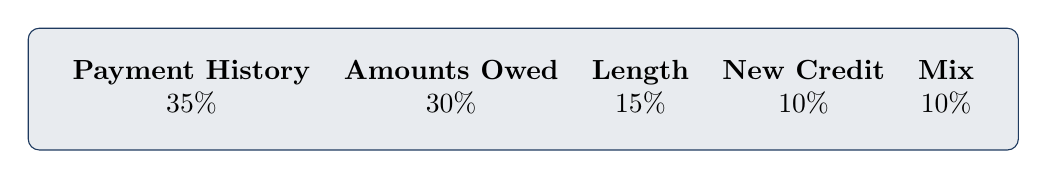
\begin{tikzpicture}
\node[draw=primaryblue, fill=primaryblue!10, rounded corners, inner sep=10pt] {
    \begin{tabular}{ccccc}
    \textbf{Payment History} & \textbf{Amounts Owed} & \textbf{Length} & \textbf{New Credit} & \textbf{Mix} \\
    35\% & 30\% & 15\% & 10\% & 10\% \\
    \end{tabular}
};
\end{tikzpicture}
\end{center}

% ============== GLOSSARY ==============
\newpage
\section*{Glossary of Abbreviations}
\addcontentsline{toc}{section}{Glossary of Abbreviations}

\begin{longtable}{lp{10cm}}
\toprule
\rowcolor{tableheader}
\textcolor{white}{\textbf{Abbreviation}} & \textcolor{white}{\textbf{Meaning}} \\
\midrule
\endhead
AAoA & Average Age of Accounts \\
AAoRA & Average Age of Revolving Accounts \\
ABORT & Average Balance on Revolving Tradelines \\
AoOA & Age of Oldest Account \\
AoORA & Age of Oldest Revolving Account \\
AoYA & Age of Youngest Account \\
AoYRA & Age of Youngest Revolving Account \\
AU & Authorized User \\
AWB & Accounts with Balance \\
AZ & All Zero \\
AZEO & All Zero Except One \\
BC & Bankcard \\
B/L & Balance to Limit (ratio) \\
BK & Bankruptcy \\
BWB & Bankcards with Balance \\
CA & Collection Agency/Authority \\
CFA & Consumer Finance Account \\
CL & Credit Limit \\
CMRRR & Certified Mail Return Receipt Requested \\
CO & Charge-off \\
CR & Credit Report \\
CRA & Credit Reporting Agency \\
DOFD & Date of First Delinquency \\
DV & Debt Validation \\
EQ & Equifax \\
EX & Experian \\
FCRA & Fair Credit Reporting Act \\
FI & Financial Institution \\
GST & Goodwill Saturation Technique \\
HELOC & Home Equity Line of Credit \\
HP & Hard Pull \\
OC & Original Creditor \\
OE & Open-ended (account) \\
PFD & Pay for Delete \\
PLOC & Personal Line of Credit \\
PR & Public Record \\
SOL & Statute of Limitations \\
SP & Soft Pull \\
SSL & Share Secured Loan \\
TCL & Total Credit Limit \\
TL & Tradeline \\
TPOD & Total Period of Delinquency \\
TU & TransUnion \\
\bottomrule
\end{longtable}

\end{document}
